\documentclass{article}

% if you need to pass options to natbib, use, e.g.:
%     \PassOptionsToPackage{numbers, compress}{natbib}
% before loading neurips_2026

% The authors should use one of these tracks.
% Before accepting by the NeurIPS conference, select one of the options below.
% 0. "default" for submission
\usepackage[preprint]{neurips_2026}
% the "default" option is equal to the "main" option, which is used for the Main Track with double-blind reviewing.
% 1. "main" option is used for the Main Track
%  \usepackage[main]{neurips_2026}
% 2. "position" option is used for the Position Paper Track
%  \usepackage[position]{neurips_2026}
% 3. "eandd" option is used for the Evaluations & Datasets Track
 % \usepackage[eandd]{neurips_2026}
% 4. "creativeai" option is used for the Creative AI Track
%  \usepackage[creativeai]{neurips_2026}
% 5. "sglblindworkshop" option is used for the Workshop with single-blind reviewing
 % \usepackage[sglblindworkshop]{neurips_2026}
% 6. "dblblindworkshop" option is used for the Workshop with double-blind reviewing
%  \usepackage[dblblindworkshop]{neurips_2026}
% 7. "education" option is used for the Education Track
%  \usepackage[education]{neurips_2026}


% After being accepted, the authors should add "final" behind the track to compile a camera-ready version.
% 1. Main Track
 % \usepackage[main, final]{neurips_2026}
% 2. Position Paper Track
%  \usepackage[position, final]{neurips_2026}
% 3. Evaluations & Datasets Track
 % \usepackage[eandd, final]{neurips_2026}
% 4. Creative AI Track
%  \usepackage[creativeai, final]{neurips_2026}
% 5. Workshop with single-blind reviewing
%  \usepackage[sglblindworkshop, final]{neurips_2026}
% 6. Workshop with double-blind reviewing
%  \usepackage[dblblindworkshop, final]{neurips_2026}
% Note. For the workshop paper template, both \title{} and \workshoptitle{} are required, with the former indicating the paper title shown in the title and the latter indicating the workshop title displayed in the footnote.
% For workshops (5., 6.), the authors should add the name of the workshop, "\workshoptitle" command is used to set the workshop title.
% \workshoptitle{WORKSHOP TITLE}
% 7. Education Track
% \usepackage[education, final]{neurips_2026}

% "preprint" option is used for arXiv or other preprint submissions
 % \usepackage[preprint]{neurips_2026}

% to avoid loading the natbib package, add option nonatbib:
%    \usepackage[nonatbib]{neurips_2026}

\usepackage[utf8]{inputenc} % allow utf-8 input
\usepackage[T1]{fontenc}    % use 8-bit T1 fonts
\usepackage{hyperref}       % hyperlinks
\usepackage{url}            % simple URL typesetting
\usepackage{booktabs}       % professional-quality tables
\usepackage{amsfonts}       % blackboard math symbols
\usepackage{nicefrac}       % compact symbols for 1/2, etc.
\usepackage{microtype}      % microtypography
\usepackage{xcolor}         % colors
\usepackage{graphicx}
\usepackage{float}

% Note. For the workshop paper template, both \title{} and \workshoptitle{} are required, with the former indicating the paper title shown in the title and the latter indicating the workshop title displayed in the footnote. 
\title{A Practical Exploration of CNNs, Vision Transformers, CLIP, and Variational Autoencoders}


% The \author macro works with any number of authors. There are two commands
% used to separate the names and addresses of multiple authors: \And and \AND.
%
% Using \And between authors leaves it to LaTeX to determine where to break the
% lines. Using \AND forces a line break at that point. So, if LaTeX puts 3 of 4
% authors names on the first line, and the last on the second line, try using
% \AND instead of \And before the third author name.


\author{%
  Zainab Amir\\
  Department of Computer Science\\
  Lahore University of Management Sciences\\
  \texttt{28100166@lums.edu.pk} \\
  % examples of more authors
  % \And
  % Coauthor \\
  % Affiliation \\
  % Address \\
  % \texttt{email} \\
  % \AND
  % Coauthor \\
  % Affiliation \\
  % Address \\
  % \texttt{email} \\
  % \And
  % Coauthor \\
  % Affiliation \\
  % Address \\
  % \texttt{email} \\
  % \And
  % Coauthor \\
  % Affiliation \\
  % Address \\
  % \texttt{email} \\
}


\begin{document}


\maketitle


\begin{abstract}
  This report explores the behaviour of several widely used deep learning architectures through a series of practical experiments involving ResNet-152, Vision Transformers, CLIP, and Variational Autoencoders. The experiments examine how pretrained representations transfer to new tasks, how residual connections and feature hierarchies affect CNN performance, how ViTs use patch-based attention and respond to missing information, and how different representations can be used for classification. The report also investigates CLIP's zero-shot capabilities and the modality gap between image and text embeddings, followed by a VAE implementation used to study latent representations, reconstruction quality, and generation on MNIST. Overall, the results highlight how architecture, pretraining objectives, and learned representations strongly influence model performance and generalization across different tasks.
\end{abstract}

\section{Introduction}

This study comprises four central experiments conducted across different fields of deep learning, with each experiment focusing on the inner workings, representations, and evaluation of a different class of models. The first concept explored is that of CNNs and transfer learning, using ResNet-152 to study feature hierarchies, feature transferability, residual connections, and their effects on classification accuracy while experimenting with both pretrained weights and random initialization.

Moving a step forward, this study then looks into Vision Transformers, with a deeper exploration of how patch-based representations and attention mechanisms work. Attention maps were extensively visualised and analysed, while additional experiments involving patch masking and alternative pooling strategies were used to study robustness and the representations learned by the model.

The third area explored is contrastive learning through CLIP, where the mode of operation of zero-shot image classification was examined using different prompting strategies. The relationship between image and text embeddings was further studied through the modality gap, followed by Procrustes alignment to investigate whether bringing the two embedding spaces closer together could improve classification performance.

Lastly, Variational Autoencoders were explored through an implementation trained on the MNIST dataset. The experiment focused on latent-space learning, reconstruction quality, and generation of new samples, while also examining how the reconstruction and KL-divergence objectives work together to learn a structured latent representation. Together, these four experiments provide a broad exploration of how different deep learning architectures learn, transfer, align, and generate representations across a range of supervised, contrastive, and generative settings.

\section{Task 1: Inner Workings of ResNet-152}
The main objective of this task was to explore the architecture of ResNet-152, a deep convolutional neural network with 152 layers, and its potential for practical applications such as transfer learning. This section details the experiments conducted to analyze components of the architecture in order to understand the inner workings of ResNet-152, with the results clearly presented and the findings explained.
\subsection{Methodology}


\subsubsection{Baseline Setup}
First, a pretrained ResNet-152 model was adapted to the CIFAR-10 dataset by replacing the original 1000-class classification layer with a 10-class linear layer. The reason we replaced only the final classification layer instead of training all 152 layers from scratch is that the pretrained model has already learned useful visual features when trained on ImageNet, and these learned features can simply be reused for the smaller CIFAR-10 dataset. Therefore, during this experiment the entire pretrained backbone was frozen, and only the classification head was trained over 3 epochs. Adam optimizer was used with a learning rate of 0.001, and the resulting training/validation loss and accuracy were recorded.

\subsubsection{Residual Connections in Practice}
Residual connections serve as an integral component of the ResNet-152 architecture.  These connections allow each layer in the model to learn a small change instead of learning the whole transformation from scratch every time \citep{he2016deep}.  This is achieved by allowing a layer's input to be added directly to its output, as follows:
\begin{equation}
    y = F(x, \{W_i\}) + x
    \label{eq:residual}
\end{equation}
where $F(x, \{W_i\})$ is the residual (the small change the model needs to learn), and $x$ is the input to the layer. 
In order to study the role these connections play in the model architecture, residual connections were disabled in three selected non-transition bottleneck blocks:
\texttt{layer1[1]}, \texttt{layer2[3]}, and \texttt{layer3[6]}.
Using the same setup as the baseline experiment earlier, the pretrained backbone remained frozen and only the final classification layer was retrained. The resulting training/validation loss and accuracy was recorded over 3 epochs, and compared with the baseline results.

\subsubsection{Feature Hierarchies and Representations}
In this section, we analyze the hierarchical representations learned by CNNs by inspecting the features collected from early, middle, and late layers of the model. The term "hierarchical" comes from how the features learned by the network build in complexity across layers, for example the earlier layers learn edges and textures while the middle layers learn combinations of shapes, leading to the final layers capturing high-level object representations.

The primary objective with this experiment is to hence determine how class separability evolves from layer to layer in such models.  To extract these representations without modifying the forward pass of the model, forward hooks were registered at three different stages of ResNet-152. These hooks allowed us to capture the intermediate activations produced as each image passed through the network, while leaving the underlying model architecture unchanged. Features were collected from an early layer, a middle layer, and a late layer, corresponding to feature dimensions of 256, 1024, and 2048 channels respectively. Since the raw convolutional outputs also contain spatial dimensions, these activations were reduced into a single feature vector for each image before visualization.

Since these feature vectors are too high-dimensional to inspect directly, t-SNE was then used to project them into a two-dimensional space. t-SNE attempts to preserve local relationships between samples, meaning that images with similar learned representations should appear closer together in the resulting plot. By applying t-SNE separately to the early, middle, and late-layer features, we can visually compare how the organization of CIFAR-10 classes changes as the representations become progressively deeper and more semantically meaningful.

\subsubsection{Transfer Learning and Generalization}
The baseline experiment helped us understand the transferability of pretrained features, but a few questions still remain unanswered. This section explores the importance of pretraining and why it matters, as well as how much of the network requires fine-tuning to achieve a good compute-accuracy trade-off.
To this end, four different experiments were set up:

\begin{itemize}
    \item Pretrained ResNet-152 with full-backbone fine-tuning
    \item Pretrained ResNet-152 with final-stage (\texttt{layer4}) fine-tuning
    \item Randomly initialized ResNet-152 with full-backbone training
    \item Randomly initialized ResNet-152 with final-stage (\texttt{layer4}) training
\end{itemize}

The same fixed subset of 5,000 training and 1,000 validation images was used across all 4 experiments, in order to ensure a controlled comparison. The number of epochs for training was also kept constant at two, and an Adam optimizer was used with the learning rate kept constant at 0.0001.

\subsection{Results}

\subsubsection{Baseline Setup}

Freezing the ResNet-152 backbone and training a new classification head for CIFAR-10 resulted in the training loss decreasing from 0.7207 to 0.4497, while the validation loss showed a smaller decrease from 0.5228 to 0.4549 in 3 epochs. On the other hand, the training accuracy increased from 78.0\% to 84.92\%, while the validation accuracy showed a similar pattern of increase, albeit of lesser magnitude, from 82.42\% to 84.38\%.


\subsubsection{Residual Connections in Practice}

The model with selected residual connections removed showed a significantly poorer performance compared to the baseline model.  As shown in Table~\ref{tab:transfer_results}, while the baseline validation accuracy increased from 82.42\% to 84.38\% across the three epochs, the no-skip connections model remained close to random guessing, only increasing from 11.66\% to 12.64\%. The validation loss also stayed almost unchanged at around 2.30, compared to the baseline loss which decreased from 0.5228 to 0.4549. This clearly shows how much the removal of residual connections, even from only a few layers, negatively impacts the model and curbs performance.

\begin{table}[h]
\centering
\begin{tabular}{lccccc}
\toprule
Model & Epoch & Train Loss & Train Acc. & Val Loss & Val Acc. \\
\midrule
Baseline & 1 & 0.7207 & 78.00\% & 0.5228 & 82.42\% \\
Baseline & 2 & 0.5000 & 83.40\% & 0.4734 & 84.10\% \\
Baseline & 3 & 0.4497 & 84.92\% & 0.4549 & 84.38\% \\
No-skip & 1 & 2.3123 & 11.45\% & 2.3033 & 11.66\% \\
No-skip & 2 & 2.3097 & 12.07\% & 2.3140 & 12.70\% \\
No-skip & 3 & 2.3092 & 11.86\% & 2.3057 & 12.64\% \\
\bottomrule
\end{tabular}
\caption{Comparison between the baseline ResNet-152 and the modified model with selected residual connections removed.}
\label{tab:transfer_results}
\end{table}

\subsubsection{Feature Hierarchies and Representations}

The t-SNE visualisation for each layer in Figure 1 shows a clear pattern. In the early layer there is a significant amount of overlap between separate classes as seen in the plot, whereas in the middle layer you can see distinct classes starting to form separate clusters. In the late layer the class separability is the most pronounced, with separate classes forming well-defined distinct clusters.
\begin{figure}[t]
    \centering

    \begin{minipage}{0.32\linewidth}
        \centering
        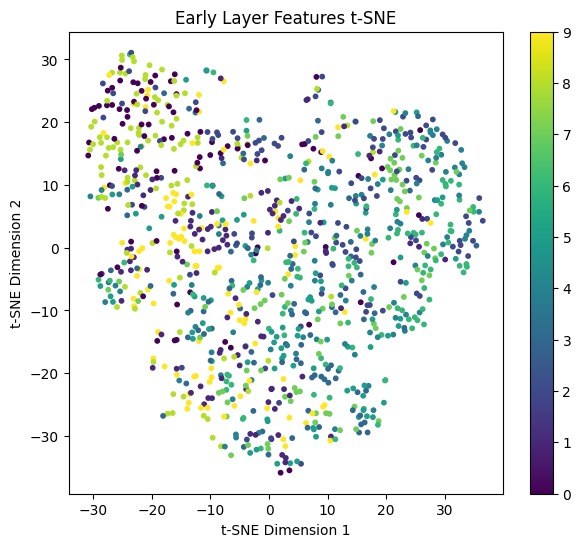
\includegraphics[width=\linewidth]{early_layer.png}
        \small (a) Early layer
    \end{minipage}
    \hfill
    \begin{minipage}{0.32\linewidth}
        \centering
        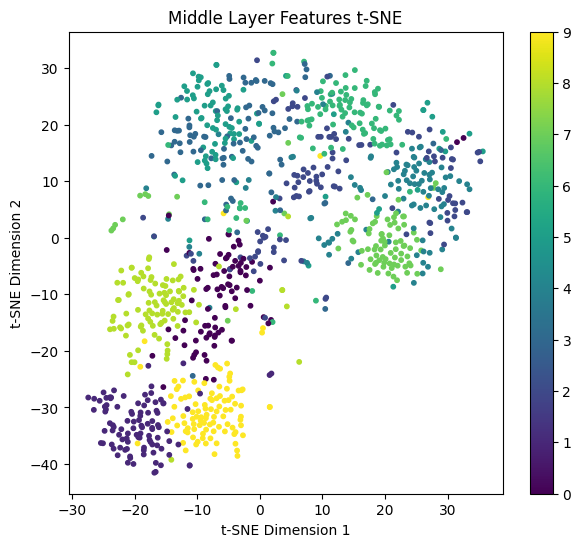
\includegraphics[width=\linewidth]{middle_layer.png}
        \small (b) Middle layer
    \end{minipage}
    \hfill
    \begin{minipage}{0.32\linewidth}
        \centering
        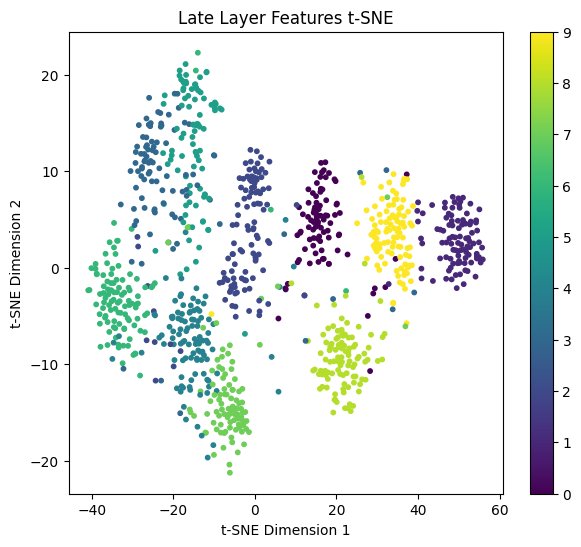
\includegraphics[width=\linewidth]{later_layer.png}
        \small (c) Late layer
    \end{minipage}

    \caption{t-SNE visualization of ResNet-152 feature representations at different network depths on CIFAR-10. }
    \label{fig:feature_hierarchy}
\end{figure}

\subsubsection{Transfer Learning and Generalization}

The ImageNet-pretrained model with only the final residual stage and classifier fine-tuned provided the best trade-off between compute and accuracy, reaching 84.9\% validation accuracy in 1.81 minutes. Although the highest accuracy was achieved by full-backbone fine-tuning, the process took a total of 4.42 minutes which is more than twice the training time. On the other hand, the full backbone trained from random initialization produced a validation accuracy of only 24.2\%, and with randomly initialized lower layers frozen, it fell even lower to 15.3\%. This shows that freezing layers is effective only when those layers already contain meaningful pretrained features.

\begin{table}[H]
\centering
\caption{Transfer learning results on CIFAR-10 using ResNet-152.}
\label{tab:transfer_results}
\begin{tabular}{l l c c}
\hline
\textbf{Initialization} & \textbf{Fine-tuning Strategy} & \textbf{Val. Accuracy} & \textbf{Training Time} \\
\hline
ImageNet pretrained & Final block + classifier & 84.9\% & 1.81 min \\
ImageNet pretrained & Full backbone & 93.9\% & 4.42 min \\
Random initialization & Full backbone & 24.2\% & 4.53 min \\
Random initialization & Final block + classifier & 15.3\% & 1.86 min \\
\hline
\end{tabular}
\end{table}

\subsection{Discussion}
\subsubsection{Baseline Setup}
Training ResNet-152 from scratch on small datasets is unnecessary and impractical because the model has a large number of parameters, and learning all these parameters would prove to be very computationally expensive, require a lot more training time, and the model would have a higher chance of overfitting as well. In this experiment, only the final classification layer was trained while the pretrained backbone remained frozen, yet the model reached 84.38\% validation accuracy after three epochs. This suggests that the visual features learned from ImageNet transfer well to CIFAR-10. The pretrained layers already capture useful general visual features, such as edges, textures, and higher-level patterns, so the new classifier mainly needs to learn how to map these features to the CIFAR-10 classes.

\subsubsection{Residual Connections in Practice}
Removing the residual connections from the three selected blocks led to a significant decline in model performance. While the baseline model achieved 84.38\% validation accuracy after three epochs, the modified model reached only 12.64\%. Its validation loss also remained close to 2.30, indicating near-random classification behavior.  This reinforces the idea that the pretrained representations depend strongly on the residual pathways through which they were learned.  Residual connections improve optimization in very deep networks by providing direct paths through which gradients can propagate during backpropagation. This helps in reducing vanishing-gradient problems and allows more efficient convergence in deeper networks. The removal of such direct pathways forces information and gradients to pass entirely through the learned transformations, making optimization more difficult. Additionally, the considerably low accuracy could also be attributed to the network being unable to adapt to the removal of the residual connections as the backbone was frozen throughout.

\subsubsection{Feature Hierarchies and Representations}
The t-SNE embeddings reveal a clear trend in class separability as depth increases through the ResNet-152 hierarchy. In the early layer, there is significant overlap amongst features for different CIFAR-10 classes, which is in line with how these layers extract generic, low-level features (edges, color gradients, textures) that are not yet class-discriminative. As we move on to the middle layer, cluster boundaries sharpen and a certain level of grouping becomes visible, reflecting how the network transitions toward mid-level representations that combine local features into object parts and shapes. The late-layer embeddings show the most distinct, well-isolated clusters with visible separation between classes. This indicates that these layers, being deeper in the network, have learned high-level, semantically meaningful representations that align closely with the classification objective. The observed pattern appears to be consistent with the broader pattern of hierarchical feature learning observed in deep CNNs.

\subsubsection{Transfer Learning and Generalization}
These results highlight the importance of pretrained representations in transfer learning. The strong performance of the pretrained models suggests that features learned on ImageNet remain useful even when transferred to a different dataset such as CIFAR-10. Fine-tuning more of the backbone allows these features to adapt further to the new task, while freezing most of the network is only useful when the frozen layers already contain meaningful representations. The poor results from the randomly initialized models further show that training such a deep network from scratch on only 5,000 images and two epochs is not sufficient to learn strong representations.


\section{Task 2: Understanding Vision Transformers}

CNNs have been used extensively in Computer Vision applications, with a major part of their success in image classification tasks being attributed to their ability of encoding useful assumptions about the input images, commonly referred to as possessing strong "inductive bias" \citep{dosovitskiy2021image}. Vision Transformers remove many of these assumptions and instead choose to rely more heavily on data to learn the visual structure, managing to match or exceed state-of-the-art CNNs on multiple image recognition benchmarks when pre-trained on sufficiently large datasets \citep{dosovitskiy2021image}. The process by which ViTs achieve this is what this section will be exploring.

\subsection{Methodology}

\subsubsection{Pre-trained ViT Classification}
Initially, a small ImageNet-pretrained ViT model, google/vit-base-patch16-224, was loaded from HuggingFace, alongside its corresponding image processor. Two images were selected, the first one showing a polar bear and the second a trolleybus, as seen in Figure~\ref{fig:attention_maps}. It must be noted that the first image had the polar bear in the centre, with barely any noise in the background while the latter did not have the trolleybus centralised and contained several elements (road, lights etc) in the background. The image processor was then used to resize and normalize the images into the expected format for the chosen model, and then each image was passed through the model for evaluation. The output logits were used to determine the highest scoring class, and the class label recorded as the top-1 prediction.

\begin{figure}[t]
    \centering

    \begin{minipage}{0.6\linewidth}
        \centering
        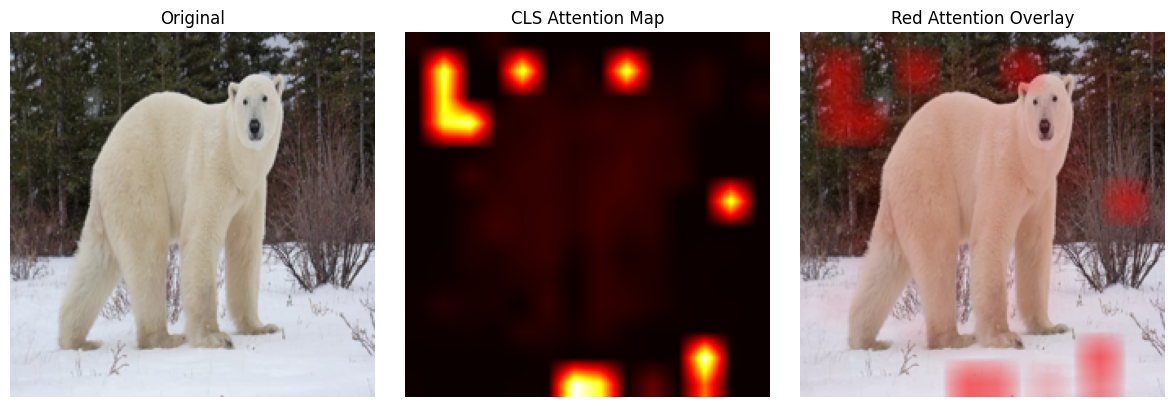
\includegraphics[width=\linewidth]{polar_bear.png}
        \small (a) Polar Bear Attention Map
    \end{minipage}
    \hfill
    \begin{minipage}{0.6\linewidth}
        \centering
        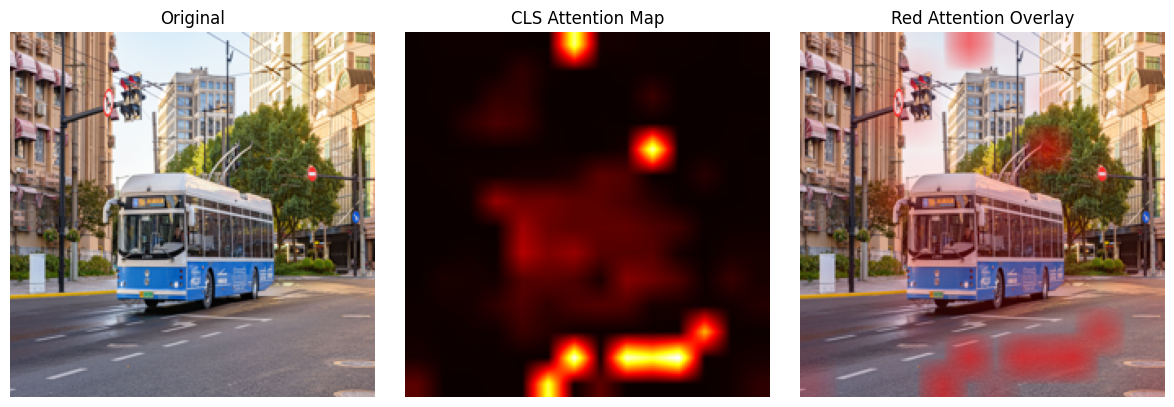
\includegraphics[width=\linewidth]{bus_attention.png}
        \small (b) Bus Attention Map
    \end{minipage}

    \caption{Final-layer CLS attention visualizations for the polar bear and bus images. The red overlay represents the relative attention intensity across image patches.}
    \label{fig:attention_maps}
\end{figure}
\subsubsection{Patch Attention Visualization}
The main objective of this section is to visualise the outputs produced by the model in the previous section using attention maps over image patches. A ViT uses self-attention in order to determine how strongly different image patches interact with each other and which regions are used for the actual classification task. For a $224 \times 224$ image using $16 \times 16$ patches:

\[
\frac{224}{16} = 14
\]

giving:

\[
14 \times 14 = 196
\]

image patches. The ViT also contains one additional [CLS] token, giving a sequence length of:

\[
196 + 1 = 197.
\]

This CLS token was particularly inspected to determine how much attention it assigned to each patch in the final transformer layer, giving us a strong idea of which regions were used for classification.

The experiment began by first configuring the model to output attention weights. The attention tensor from the final layer had the shape $[2, 12, 197, 197]$, corresponding to the number of images, number of attention heads, and sequence lengths respectively. The attention originating from the CLS token was then selected, after which the 12 attention heads were averaged together to produce a single attention vector for each image. The resulting attention values were reshaped into a $14 \times 14$ attention map, which was then displayed as a semi-transparent overlay on the original image, with stronger red regions representing higher attention weights.

\subsubsection{Patch-Masking Experiment}
A patch-masking experiment was conducted to test the robustness of the model, employing two different types of masking strategies:

\begin{itemize}
    \item Random patch masking
    \item Structured centre patch masking

\end{itemize}

In both cases a fixed 25\% of the total image patches were masked, which resulted in a total of 49 patches being masked per image as each image was divided into \[14 \times 14 = 196\] patches. In the case of random masking, 49 random patch locations were selected across the image, while for structured centre patch masking a central block of \[7 \times 7\] patches was removed after the necessary calculations. The same pretrained model was then used to classify each set of images, with the resulting class predictions and confidence scores being used to compare the effect of each masking strategy on model performance.



\subsubsection{CLS Token vs. Mean-Pooled Patch Tokens}
For this experiment, the representations produced by the pretrained ViT were compared using two different pooling approaches. The first used the final [CLS] token as the image representation, while the second used the mean of all patch-token representations from the final transformer layer.  Features were extracted for a subset of 5,000 CIFAR-10 training images and 1,000 test images, with the pretrained ViT kept fixed throughout the experiment. A separate linear classifier was then trained on each set of 768-dimensional features for 20 epochs, and the resulting training and test accuracies were compared to determine which representation provided more useful information for classification.


\subsection{Results}

\subsubsection{Pre-trained ViT Classification}

The pre-trained ViT correctly classified both test images. For the first image the model predicted ``ice bear, polar bear, Ursus Maritimus, Thalarctos maritimus'', while for the second the prediction was ``trolleybus, trolley coach, trackless trolley''. In both cases, the top-1 prediction matched the main object present in the image, indicating that the ImageNet-pretrained model was able to correctly identify both examples without any additional training.

\subsubsection{Patch Attention Visualization}


The final-layer attention tensor had a shape of $[2, 12, 197, 197]$, corresponding to the two input images, 12 attention heads, and 197 tokens consisting of one class token and 196 image patches. 

As shown in Figure~\ref{fig:attention_maps}, the strongest attention for the polar bear image was distributed across several different parts of the background, with only minimum to moderate attention being given to the main polar bear at the centre. On the other hand, for the trolleybus image stronger attention was directed towards the road, but significant attention was also given to the bus itself, visibly more apparent than the polar bear.

As shown in Figure~\ref{fig:attention_maps2}, the individual attention heads also showed noticeably different patterns, with some heads focusing on relatively small regions while others showed broader attention across the image.

\begin{figure}[t]
    \centering

    \begin{minipage}{0.48\linewidth}
        \centering
        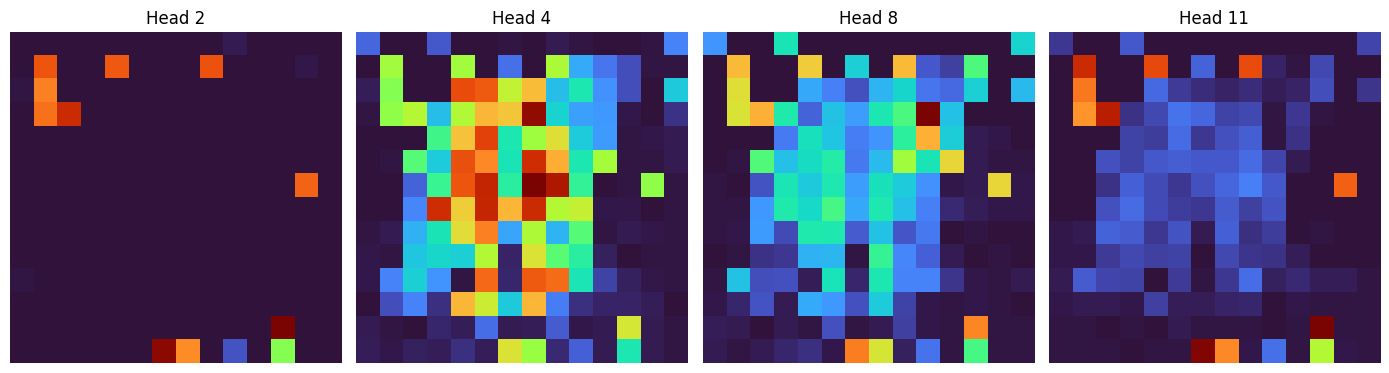
\includegraphics[width=\linewidth]{bear_heads.png}
        \small (a) Polar Bear Attention Heads
    \end{minipage}
    \hfill
    \begin{minipage}{0.48\linewidth}
        \centering
        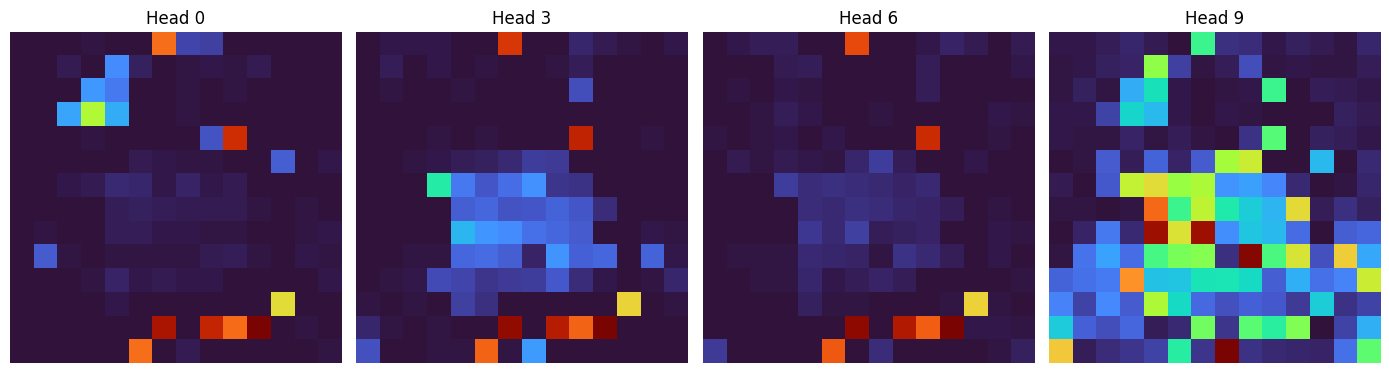
\includegraphics[width=\linewidth]{bus_heads.png}
        \small (b) Bus Attention Heads
    \end{minipage}

    \caption{Multiple Attention Heads}
    \label{fig:attention_maps2}
\end{figure}

\subsubsection{Patch Masking}

As shown in Table~\ref{tab:patch_masking}, the polar bear prediction remained highly stable after both random and structured patch masking. The original prediction had a confidence of 99.91\%, while randomly masking 25\% of the patches resulted in a confidence of 99.89\%. When the central 25\% of patches were masked, the model still predicted polar bear with a confidence of 99.32\%.

The trolleybus image showed a considerably larger change under the same conditions. The original trolleybus prediction had a confidence of 98.82\%, which decreased to 72.82\% after random patch masking. With the central patches masked, the top-1 prediction changed from trolleybus to traffic light with a confidence of 57.44\%.

\begin{figure}[t]
    \centering

    \begin{minipage}{0.48\linewidth}
        \centering
        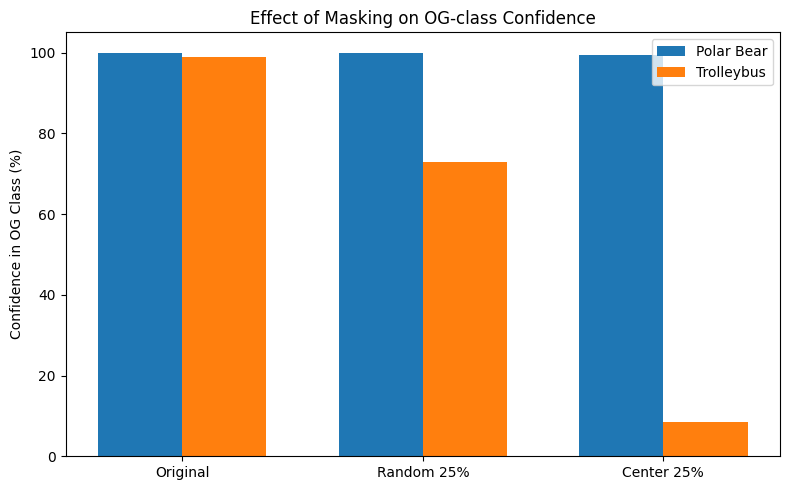
\includegraphics[width=\linewidth]{25_maskingg.png}
        \small (a) Effect of Patch Masking on predictions
    \end{minipage}
    \hfill
    \begin{minipage}{0.48\linewidth}
        \centering
        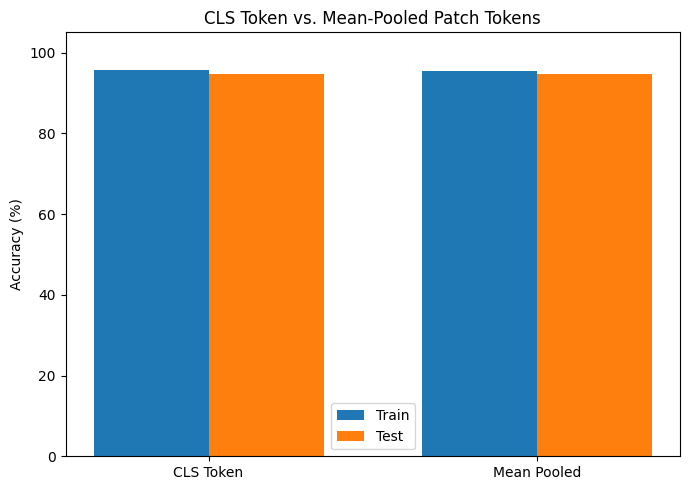
\includegraphics[width=\linewidth]{cls.png}
        \small (b) CLS Token vs Mean-Pooled
    \end{minipage}
    \caption{Patch Masking and Pooling Strategies}
    \label{fig:masking}
\end{figure}


\begin{table}[t]
\centering
\caption{Effect of patch masking on ViT predictions.}
\label{tab:patch_masking}
\begin{tabular}{lccc}
\hline
Image & Original & Random 25\% & Center 25\% \\
\hline
Polar Bear & 99.91\% & 99.89\% & 99.32\% \\
Trolleybus & 98.82\% & 72.82\% & Traffic Light (57.44\%) \\
\hline
\end{tabular}
\end{table}

\subsubsection{CLS Token vs Mean-Pooled Patch Features}

As shown in Table~\ref{tab:linear_probe} and Figure~\ref{fig:masking}(b), the two representations produced very similar performance when used to train linear classifiers on CIFAR-10. The classifier trained using the CLS token achieved a training accuracy of 95.56\% and a test accuracy of 94.60\%, while the classifier using mean-pooled patch tokens achieved a training accuracy of 95.30\% and a slightly higher test accuracy of 94.80\%.

Although the CLS token achieved a slightly higher training accuracy, the difference between the two representations on the test set was only 0.20 percentage points, showing that both representations contained similarly useful information for CIFAR-10 classification.

\begin{table}[t]
\centering
\caption{Linear probe performance using CLS and mean-pooled patch representations.}
\label{tab:linear_probe}
\begin{tabular}{lcc}
\hline
Representation & Training Accuracy & Test Accuracy \\
\hline
CLS Token & 95.56\% & 94.60\% \\
Mean-Pooled Patches & 95.30\% & 94.80\% \\
\hline
\end{tabular}
\end{table}


\subsection{Discussion}

\subsubsection{Patch Attention Analysis}
The attention maps show that the model did not rely exclusively on the main object when making its predictions. In the case of the polar bear image, a significant amount of attention was directed towards the surrounding background, whereas the trolleybus image showed comparatively higher intensity attention on both the object and contextual regions such as the road. 

This, however, does not imply that the object was ignored entirely, because the visualization in Figure~\ref{fig:attention_maps} only shows the final-layer CLS-to-patch attention and does not represent all the information used by the model to classify the images. By the final layer, the patch representations have repeatedly exchanged information and it is probable that a patch receiving high final attention may contain information originating from the main object itself. Apart from that, the model may also be using contextual cues for classification such as the snowy background surrounding the polar bear, or the road and traffic surrounding the bus. This suggests that the ViT can make use of both object-specific information and the broader context of an image during classification.

As shown in Figure~\ref{fig:attention_maps2}, a few additional attention maps were generated to study individual attention heads, resulting in markedly different patterns for different heads. Some of the heads focused on smaller, localized regions, while others showed a broader distribution of attention across the image. This suggests that some level of specialization may be occurring between the different heads, as each head can learn to capture different relationships between patches.

Attention-based visualisation also differs from CNN interpretation methods such as CAM or Grad-CAM. In a ViT, the attention weights are produced directly during the forward pass and can therefore be inspected without requiring an additional gradient-based procedure. Grad-CAM, on the other hand, uses gradients flowing through intermediate convolutional feature maps to determine which regions contributed to a particular prediction \cite{selvaraju2017gradcam}. This gives transformers a convenient built-in mechanism for examining interactions between image patches, although attention intensity should not necessarily be interpreted as a direct measure of how important a region was to the final prediction.



\subsubsection{Patch-Masking Experiment}
Our results for the patch-masking experiment show how robustness can be highly dependent on the image being used as input even with the same masking strategy applied. In the case of the polar bear image, the model remained highly robust to patch removal and maintained the correct class for both random and center masking, which could possibly be attributed to how the bear’s body and shape extend across several different patches. For example, the bear’s defining facial features remain above the central masked region, which could explain the robustness to centre patch masking. On the other hand, the bus image was less robust as random masking preserved the trolleybus prediction but reduced confidence from 98.82\% to 72.82\%, while center masking changed the prediction to a traffic light at 57.44\%. This suggests that structured masking can be more damaging when it removes a contiguous region containing the main object, such as a major part of the vehicle in the case of the trolleybus image, whereas random masking preserves distributed object evidence across the image.


\subsubsection{CLS Token vs. Mean-Pooled Patch Tokens}
The very similar performance of the CLS-token and mean-pooled patch representations suggests that useful global information was present in both by the final transformer layer. The CLS token is directly used for classification during ViT pretraining, which may explain its slightly higher training accuracy, while repeated self-attention also allows patch tokens to exchange information and become strong global representations when averaged. The very small difference in test accuracy suggests that neither pooling method was clearly superior in this experiment. This is also consistent with the original ViT paper, which found that class-token and global-average-pooling classifiers could perform comparably when optimized appropriately.

\section{Task 3: CLIP Tasks}

\subsection{Methodology}

\subsubsection{Zero-Shot Classification on STL-10}
This experiment aimed to evaluate the zero-shot classification accuracy of CLIP on the STL-10 dataset from Torchvision. The pretrained OpenAI CLIP ViT-B/32 model was used to evaluate the dataset, with three prompting strategies used during evaluation:

\begin{itemize}
    \item Plain class labels: ``[class]''
    \item Prompted text: ``a photo of a [class]''
    \item Descriptive prompts: class-specific short descriptions, e.g., ``a photo of a horse in a field''
\end{itemize}

Before being passed through the model, the images and prompts were prepared separately, with each image being processed and encoded while each prompt was tokenized and encoded as well. The similarity between the resulting image and text embeddings was then computed using the dot product:

\[
s(i,t) = \mathbf{v}_i^\top \mathbf{t}
\]

where $\mathbf{v}_i$ represents the image embedding and $\mathbf{t}$ represents the text embedding.

Finally, the class with the highest similarity score was selected as the prediction, and the resulting classification accuracies were recorded for comparison across the three prompting strategies.

\subsubsection{Exploring the Modality Gap}
The main objective of CLIP is to align images and text, but have we considered whether their embeddings actually occupy the same region of space? Instead of forcing the embeddings for an image and its corresponding text to be identical, CLIP's contrastive objective encourages matching image-text pairs to have higher similarity than mismatched pairs \citep{radford2021clip}. Therefore, image and text embeddings may still form separate clouds or clusters while preserving the relative similarities required for classification, which is termed the ``modality gap''.

In order to examine this modality gap, an experiment was conducted using a subset of 50 STL-10 test images. Each image was encoded using the pretrained CLIP ViT-B/32 image encoder, while its corresponding class prompt was encoded using the CLIP text encoder. Since the resulting embeddings are high-dimensional, t-SNE was then used to project both modalities into a two-dimensional space for visual comparison. The image and text embeddings were visualised both before and after normalization in order to determine whether normalization affected the separation between the two modalities.
\begin{figure}[t]
    \centering
    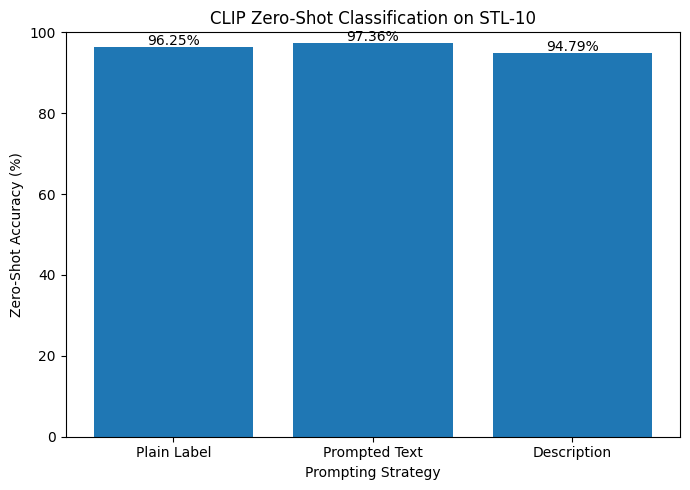
\includegraphics[width=0.5\linewidth]{prompt.png}
    \caption{Zero-Shot Accuracy for The Three Prompting Strategies}
    \label{clip_prompt}
\end{figure}
\subsubsection{Bridging the Modality Gap}
This experiment was focused on reducing the previously introduced modality gap between CLIP image and text representations using orthogonal Procrustes alignment. The alignment was applied to the normalized embeddings from 50 paired STL-10 image-text samples, with the image embeddings $X$ and their corresponding text embeddings $Y$ each having dimensionality $50 \times 512$.

The objective of orthogonal Procrustes alignment is to find an orthogonal rotation matrix $R$ that minimizes the Frobenius distance between the transformed image embeddings and the corresponding text embeddings:

\[
R^* = \arg\min_{R} \|XR - Y\|_F
\]


where $\|\cdot\|_F$ denotes the Frobenius norm. 


The optimal rotation matrix was learned using \texttt{scipy.linalg.orthogonal\_procrustes}, and the aligned image representations were then computed as:

\[
X_{\text{aligned}} = XR,
\]


The aligned image and text embeddings were visualized using t-SNE. The same learned rotation matrix was then applied to the image embeddings from the complete STL-10 test set, and then finally, zero-shot classification was performed using the prompted-text strategy from Task 3.1. 


\subsection{Results}

\subsubsection{Zero-Shot Classification on STL-10}



As shown in Figure~\ref{clip_prompt}, CLIP achieved strong zero-shot classification performance across all three prompting strategies. Using plain class labels resulted in an accuracy of 96.25\%, while using the prompted text format ``a photo of a [class]'' increased the accuracy to 97.36\%. On the other hand, the more descriptive prompting strategy resulted in a lower accuracy of 94.79\%. Among the three approaches, the prompted text strategy therefore produced the highest zero-shot classification accuracy on the STL-10 test set.

\subsubsection{Exploring the Modality Gap}

\begin{figure}[t]
    \centering

    \begin{minipage}{0.48\linewidth}
        \centering
        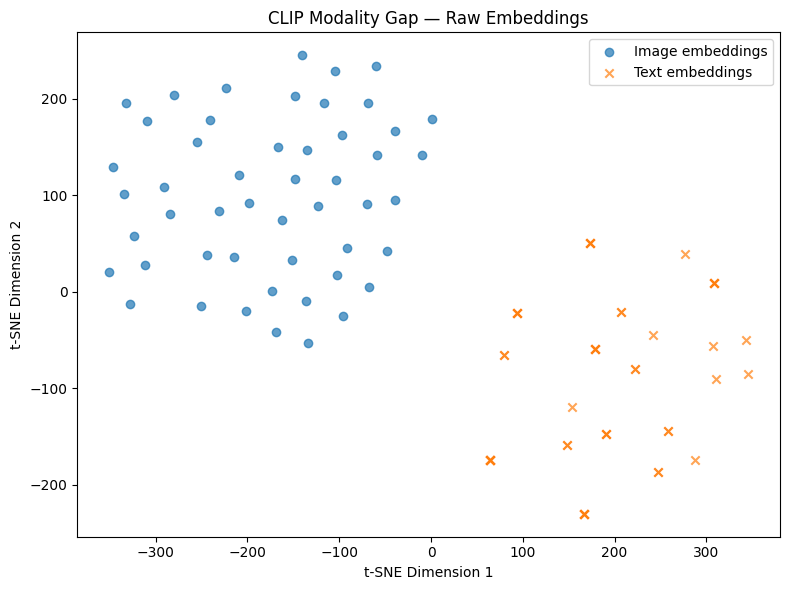
\includegraphics[width=\linewidth]{32_modgap.png}
        \small (a) CLIP Modality Gap for Raw Embeddings
    \end{minipage}
    \hfill
    \begin{minipage}{0.48\linewidth}
        \centering
        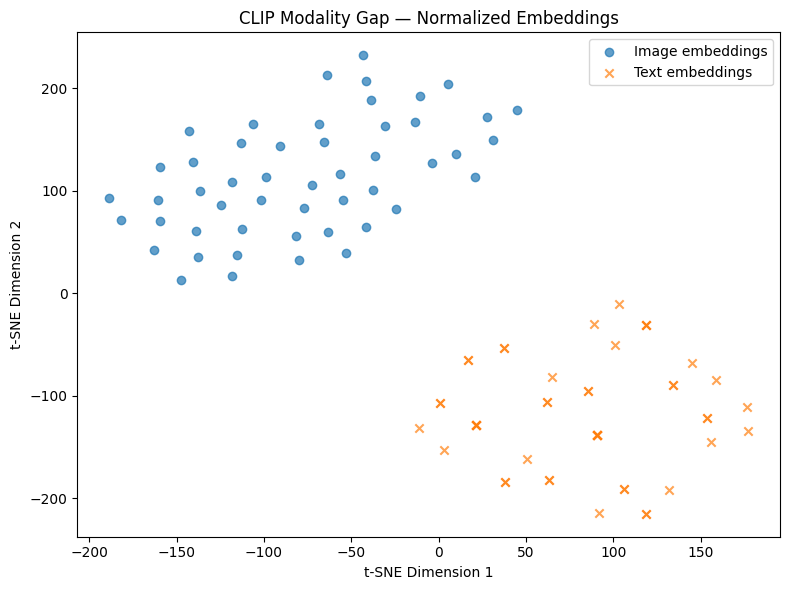
\includegraphics[width=\linewidth]{32_modnorm.png}
        \small (b) CLIP Modality Gap for Normalized Embeddings
    \end{minipage}

    \caption{CLIP Modality Gap using t-SNE}
    \label{fig:modality_gap}
\end{figure}

As shown in Figure~\ref{fig:modality_gap}(a), the image and text embeddings occupied visibly different regions of the t-SNE space, showing a clear separation between the two modalities. This separation continued to remain visible even after normalizing the embeddings as seen in Figure~\ref{fig:modality_gap}(b), although normalization removed differences in their magnitudes. Before normalization, the mean norm of the image embeddings was 10.56, compared to 10.14 for the text embeddings.

\subsubsection{Bridging the Modality Gap}

\begin{figure}[t]
    \centering
    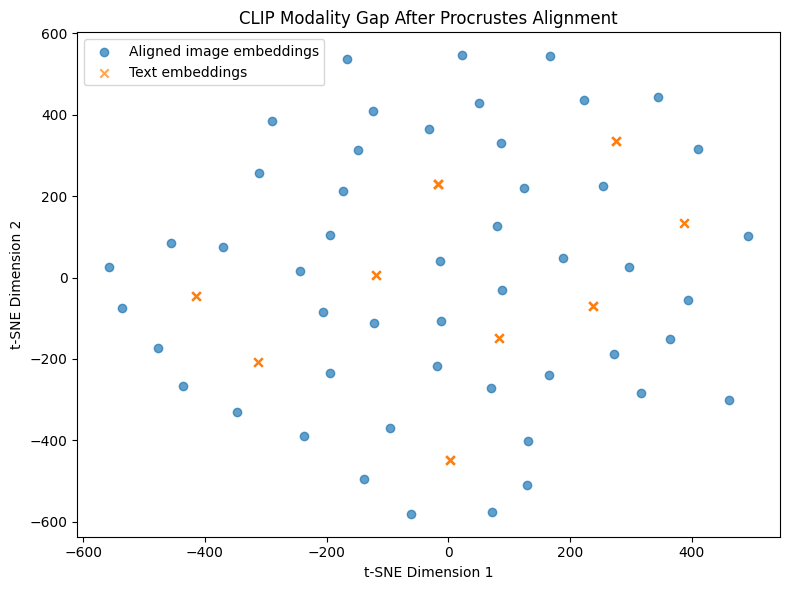
\includegraphics[width=0.5\linewidth]{modgap_procrustes.png}
    \caption{Modality Gap After Procrustes Alignment}
    \label{procrustes_align}
\end{figure}

Applying the orthogonal Procrustes transformation resulted in a significant reduction of the distance between the paired image and text embeddings. The Frobenius error decreased from 8.57 before alignment to 3.42 after alignment, while the t-SNE visualization in Figure~\ref{procrustes_align} also showed the two modalities becoming more closely aligned.

However, notably this improvement in geometric alignment did not result in better zero-shot classification performance. Using the original prompted-text embeddings produced an accuracy of 97.36\%, whereas applying the learned Procrustes transformation to the image embeddings reduced the accuracy to 86.44\% - a total decrease of 10.92 percentage points.

\subsection{Discussion}
\subsubsection{Zero-Shot Classification on STL-10}
Since CLIP classifies images by comparing image embeddings with text embeddings, changing the wording of the prompt changes the resulting class representation in the shared embedding space. The results show the various ways in which prompting strategies affect CLIP’s zero-shot performance. The prompted text strategy “ a photo of a [class]” produced the highest accuracy, which could possibly be explained by how the prompt provides just enough useful context of the image for the model without excess noise. On the other hand, the descriptive prompts performed worse, indicating how additional details can interfere with the model’s classification abilities. For example, “ a photo of a horse in the field” may be less suitable for images of horses without a field. All in all, this experiment showed how simple prompts may work better than excessive descriptions for zero-shot CLIP classification.

\subsubsection{Exploring the Modality Gap}
The results show t-SNE plots with a clear modality gap between CLIP image and text embeddings in both the raw and normalized representations. The gap remaining clearly visible after L2 normalization helps us verify that the modality gap shown was not caused by differences in embedding magnitudes. This is further reinforced by the fact that the mean L2 norms of the raw image and text embeddings were similar at 10.56 and 10.14 respectively.

We can thus infer that the modality gap likely reflects differences in the orientation and structure of image and text representations within CLIP's embedding space. However, despite this separation, the strong zero-shot classification performance shows that the two modalities can still remain sufficiently aligned for similarity-based matching, which is consistent with prior observations of a persistent modality gap in multimodal contrastive models \citep{liang2022mind}.

\subsubsection{Bridging the Modality Gap}
The results show that reducing the geometric distance between image and text embeddings does not necessarily improve CLIP's zero-shot performance. While the Procrustes alignment was able to successfully reduce the Frobenius error from 8.57 to 3.42, it also led to a change in the geometry of the image embedding space relative to the text embeddings used for classification.

This suggests that CLIP does not require the two modalities to perfectly overlap, as its contrastive objective mainly encourages matching image-text pairs to be more similar than incorrect pairs as detailed earlier. A probable explanation for the drop in accuracy from 97.36\% to 86.44\% would be that forcing the embeddings closer disrupted some of the similarity structure originally learned by CLIP. Thus, Procrustes alignment managed to reduce the modality gap but led to a decrease in classification accuracy instead of a possible increase. Additionally, the small alignment sample, containing only nine distinct target text embeddings, may also have contributed to this decrease in classification accuracy.


\section{Task 4: Variational Autoencoder}

\subsection{Methodology}
\subsubsection{Building a Basic VAE}
In this experiment, a Variational Autoencoder was implemented in PyTorch and trained on the MNIST dataset. Each $28 \times 28$ image was first flattened into a 784-dimensional vector and passed through a fully connected hidden layer containing 400 units. The encoder then produced a 2-dimensional mean $\mu$ and log-variance $\log \sigma^2$, which parameterized the Gaussian latent distribution. A latent vector $z$ was sampled using the reparameterization trick \citep{kingma2014autoencoding}, which is as follows:

\[
z = \mu + \sigma \odot \epsilon,
\qquad \epsilon \sim \mathcal{N}(0,I).
\]

The vector was then passed through the decoder, consisting of another 400-unit hidden layer and a 784-dimensional output layer used to reconstruct the original image. Afterwards, pixel probabilities were calculated by applying a sigmoid activation to the final output.

The model was trained using the VAE loss, consisting of a binary cross-entropy reconstruction loss and a KL-divergence term for regularization purposes. The Adam optimizer with a learning rate of $0.001$ was used, and the model was trained for 10 epochs while monitoring the total, reconstruction, and KL losses.

\begin{figure}[t]
    \centering

    \begin{minipage}{0.48\linewidth}
        \centering
        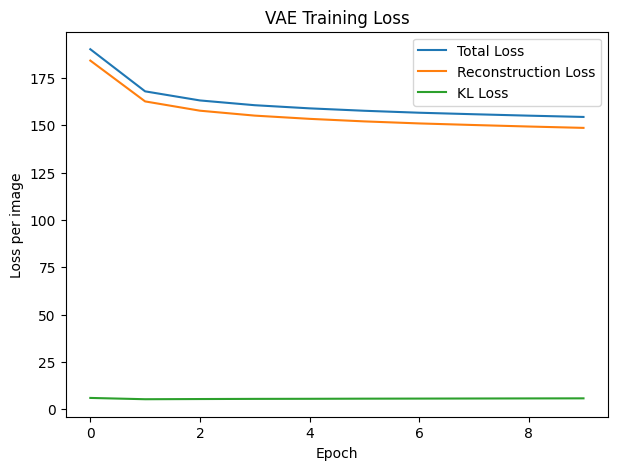
\includegraphics[width=\linewidth]{41_trloss.png}
        \small (a) VAE Training Loss 
    \end{minipage}
    \hfill
    \begin{minipage}{0.48\linewidth}
        \centering
        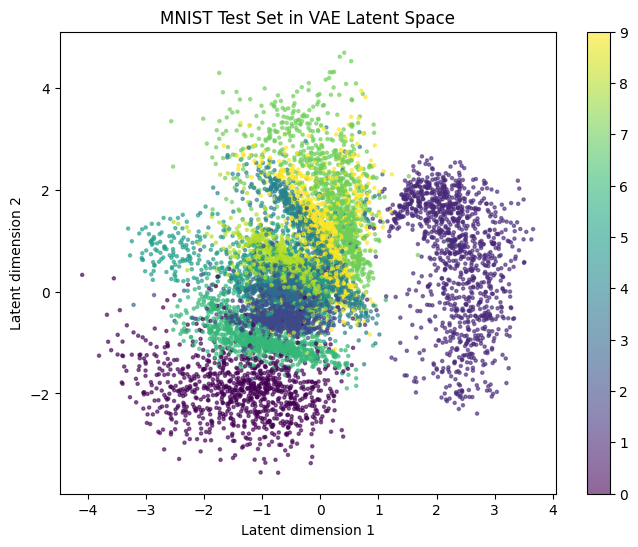
\includegraphics[width=\linewidth]{42_latentspace.png}
        \small (b) MNIST Test Set in VAE Latent Space
    \end{minipage}

    \caption{VAE training loss and learned latent-space representation.}
    \label{fig:vae_training}
\end{figure}

\subsubsection{Analyzing VAE Performance}
The main objective was to evaluate the trained VAE through three different experiments:

\begin{itemize}
    \item \textbf{Latent-space visualization:} MNIST test images were passed through the encoder and the mean vector, $\mu$, was used as the latent representation. Since the latent dimension was two, further dimensionality reduction was not needed and the embeddings could be plotted directly, with points coloured according to their true digit labels.

    \item \textbf{Reconstruction quality:} A random sample of 8 images was taken from the MNIST dataset and passed through the VAE. The reconstructed outputs were displayed and compared with the original images so that visual differences between the two could be noted and reconstruction quality gauged.

    \item \textbf{Random sample generation:} Random latent vectors were sampled directly from the prior distribution $z \sim \mathcal{N}(0,I)$ and passed through the decoder without any input images to generate new digit images. The outputs were then displayed to check whether the model was capable of generating realistic handwritten digits.
\end{itemize}

\subsection{Results}

\subsubsection{VAE Training}



As shown in Figure~\ref{fig:vae_training}(a), the total VAE loss decreased steadily over the 10 training epochs, from 190.19 in the first epoch to 154.42 in the final epoch. The reconstruction loss followed a similar pattern, decreasing from 184.19 to 148.64, while the KL divergence remained comparatively stable around 5--6 throughout training. 

\subsubsection{Analyzing VAE Performance}

As shown in Figure~\ref{fig:vae_training}(b), the two-dimensional latent space showed how some of the MNIST digit classes formed relatively distinct regions, while a significant amount of overlap remained between others, particularly around the centre of latent space. This shows that the VAE learned an organized representation of the digits without separating each class into completely distinct clusters.

The reconstructions shown in Figure~\ref{fig:vae_analysis}(a) were able to retain the general structure of the original digits, although they appeared noticeably blurrier. While most of the reconstructed digits remained recognizable, some examples differed from their original inputs as apparent in the figure.

Finally, as shown in Figure~\ref{fig:vae_analysis}(b), samples drawn randomly from the latent prior produced images resembling handwritten digits. Several generated samples were clearly recognizable, while others appeared more ambiguous with characteristics that could correspond to more than one digit class.



\subsection{Discussion}
\subsubsection{VAE Training}
Overall, the decrease in total and reconstruction loss shows that during training the model was able to gradually improve its ability to reconstruct the MNIST images by learning a useful latent representation. On the other hand, the KL divergence remained relatively stable because it acts as a regularization term, encouraging the learned latent distribution to remain close to the standard normal prior rather than directly improving reconstruction quality. Any small fluctuations or the observed slight increase can therefore be attributed to the model balancing better reconstruction while attempting to maintain a well-structured latent space.

\subsubsection{Analyzing VAE Performance}
The latent-space visualization shows how the VAE learned meaningful representations despite not being trained explicitly for classification. The objective was not class separation, which helps explain the overlap between digit classes, as the VAE was primarily trained for digit reconstruction and latent regularization. Secondly, the reconstructions obtained were quite blurry, which can partly be explained by compressing a 784-dimensional image into only two latent variables. This strong compression can result in the loss of finer structural details, contributing to the blurriness observed in the reconstructed digits and a few errors, such as reconstructing the digit 4 as 9. The VAE objective itself can also favour smoother reconstructions rather than preserving every fine detail.

Lastly, in the third experiment, the model was able to generate recognizable digits from randomly sampled latent vectors. This suggests that the latent space was successfully regularized toward the standard normal prior, allowing samples drawn from previously unseen points in the latent space to still produce meaningful digit-like outputs.

\begin{figure}[t]
    \centering

    \begin{minipage}{0.48\linewidth}
        \centering
        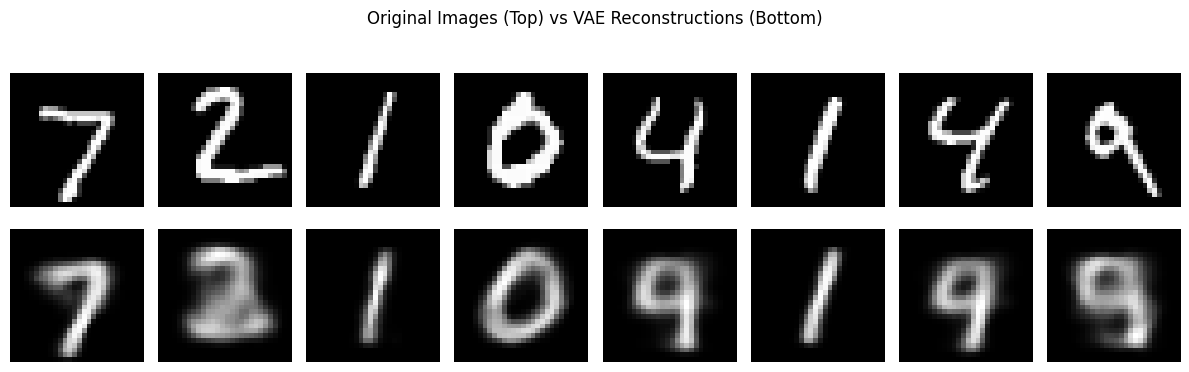
\includegraphics[width=\linewidth]{42_recon.png}
        \small (a) Reconstructed Digits
    \end{minipage}
    \hfill
    \begin{minipage}{0.48\linewidth}
        \centering
        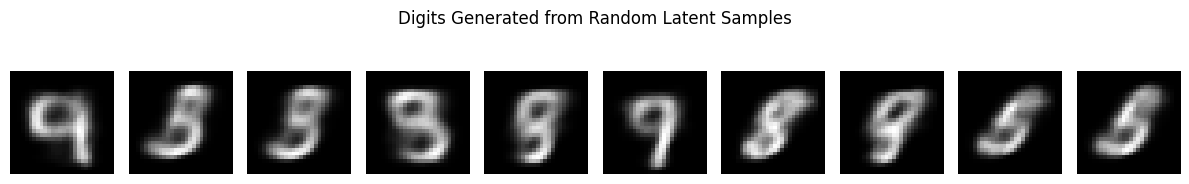
\includegraphics[width=\linewidth]{42_generate.png}
        \small (b) Generated Digits
    \end{minipage}

    \caption{Reconstructed and Generated Digits}
    \label{fig:vae_analysis}
\end{figure}

\subsubsection{Comparing with Doersch’s VAE Implementation:}

\textbf{Architecture:} 
The VAE implemented in this task uses a fully connected architecture. Each $28 \times 28$ MNIST image is first flattened into a 784-dimensional vector and passed through a hidden layer containing 400 units with ReLU nonlinearities. The encoder then produces a 2-dimensional mean $\mu$ and log-variance $\log \sigma^2$, which are used to sample the latent representation. The decoder takes this sampled latent vector and passes it through another 400-unit hidden layer, again using a ReLU nonlinearity, before reconstructing the original 784-dimensional input.

Doersch's implementation follows a very similar overall VAE structure, where the encoder parameterizes a Gaussian latent distribution and the decoder reconstructs the input from the sampled latent representation. ReLU nonlinearities are also used within the hidden layers, making the overall architecture broadly similar to the one implemented in this experiment.

\textbf{Output Distribution and Loss:}
Doersch's tutorial uses a sigmoid cross-entropy loss, similar to the binary cross-entropy used in this implementation. In both cases, the MNIST pixel values are treated as probabilities under a Bernoulli output distribution, with the decoder producing values between 0 and 1 through a sigmoid activation. Therefore, the output distribution and loss used in our VAE closely match those described by Doersch.

\textbf{Latent Dimensionality:}

A 2-dimensional latent space was used in this experiment, mainly to allow direct visualization without additional dimensionality reduction. The resulting latent plot showed meaningful structure, although several digit classes overlapped. Doersch notes that VAE performance is generally not highly sensitive to latent dimensionality over a reasonable range, except when the latent space is extremely small or large.

\textbf{Results Comparison:}

Doersch's VAE produced mostly realistic digits with a few ambiguous exceptions, and this implementation followed a similar pattern by producing recognizable but slightly blurry reconstructions. A few "failure cases" were observed, with the digit 4 being reconstructed as a shape resembling the digit 9 in two cases. This was quite similar to Doersch's case, where one of the reported failure cases involved a sample appearing to be a blend of the digits 7 and 9.


\section{Conclusion}
Through a series of experiments conducted across four different areas of deep learning, this study explored and analyzed important training and evaluation processes employed by various models from ResNet-152 and Vision Transformers to CLIP and Variational Autoencoders. The inner mechanisms of each model were studied from multiple angles including feature transfer, residual connections, attention, robustness, multi-modal representations, and latent-space learning. Overall, the experiments provided a broad understanding of how different supervised, self-supervised, and generative learning approaches develop and use learned representations for different downstream tasks.

\bibliographystyle{plainnat}
\bibliography{references}


\end{document}